\documentclass[11pt,a4paper]{ctexart}
\usepackage[margin=2.5cm]{geometry}
\usepackage{graphicx}
\usepackage{booktabs}
\usepackage{longtable}
\usepackage{hyperref}
\usepackage{caption}
\hypersetup{colorlinks=true,linkcolor=blue,citecolor=blue,urlcolor=blue}
\captionsetup{labelfont={bf},font=small}
\title{大颗粒原煤 LIBS 光谱的多示例学习热值校准预测\\
\large 5 折交叉验证复现报告}
\author{格物科学智能体 (gewu)\\基于 coal 复现实验}
\date{2026-10-28}

\begin{document}
\maketitle
\tableofcontents
\newpage

\section{摘要}
本报告基于多示例学习（Multiple Instance Learning, MIL）对激光诱导击穿光谱（LIBS）大颗粒原煤做端到端热值（Gross Calorific Value, GCV）校准预测。方法采用 \texttt{sg $\rightarrow$ als $\rightarrow$ mms} 三级预处理、ResNet1D 编码器 + SupCon 预训练、TransMIL 注意力聚合与 FiLM 融合，并以 PLSR 基线 + MIL 残差修正构成 \emph{hybrid} 融合预测。5 折 bag 级交叉验证（每折验证集 14 个 bag）给出 hybrid RMSE 均值 $214.57 \pm 25.71$ kcal/kg（$0.8978 \pm 0.1076$ MJ/kg），全部 5 折 RMSE 与外部项目官方 \texttt{summary.json} 交叉校验一致（官方均值 214.5699 vs 本地重算 214.5699 kcal/kg，绝对差 $1.1\times 10^{-5}$），核心数值可复现。

\section{方法}
\subsection{光谱预处理（sg $\rightarrow$ als $\rightarrow$ mms）}
大颗粒原煤 LIBS 谱受基线漂移、散粒噪声与量纲差异影响，按三级流水线处理：
\begin{enumerate}
  \item Savitzky--Golay（\texttt{sg}）平滑：去除高频随机噪声；
  \item 自适应最小二乘基线校正（\texttt{als}）：消除连续背景与基线漂移；
  \item Min-Max 归一化（\texttt{mms}）：把谱强度映射到 $[0,1]$，消除激光能量波动带来的量纲差异。
\end{enumerate}
三步串行作用于每条原始光谱，得到下游建模用的归一化谱。

\subsection{模型架构}
\begin{itemize}
  \item \textbf{编码器}：ResNet1D（base 通道数 16）+ SupCon 自监督预训练，从一维 LIBS 谱提取抗噪表征；
  \item \textbf{聚合}：TransMIL 注意力机制在 bag 内对多示例（多张谱）做加权聚合，得到 bag 级表征；
  \item \textbf{融合}：FiLM（Feature-wise Linear Modulation），\texttt{plsr\_dim=7}，将 PLSR 线性先验嵌入残差支路，构成 hybrid 融合。
\end{itemize}
总参数规模 $n_{\text{total}} = 924{,}895$。\texttt{method} 标签为 \texttt{pretrain+TransMIL\_attn}。

\subsection{hybrid 融合预测策略}
hybrid = PLSR 基线预测 + MIL 残差修正。PLSR 提供线性可解释基线，TransMIL 学习谱—热值的非线性残差，FiLM 在特征层完成两路信息融合。该结构在保证可解释性的同时提升大颗粒原煤的泛化精度。

\subsection{5 折 bag 级交叉验证}
全部 bag 随机划分为 5 折；每轮取 1 折作验证集、其余 4 折作训练集。验证以 bag 为单位拆分（而非以单张谱为单位），避免同一 bag 的谱同时落入训练与验证，保证评估无信息泄漏。每折验证集 $n = 14$ bag。

\section{实验设置}
\subsection{数据}
对象为大颗粒原煤 LIBS 光谱，每个 bag 对应一份原煤样品的多张光谱，标签为该样品的实际热值（kcal/kg）。光谱经 sg $\rightarrow$ als $\rightarrow$ mms 预处理后进入模型。

\subsection{折划分与训练配置}
\begin{itemize}
  \item 交叉验证折数：5；每折验证 bag 数：14；
  \item 编码器：ResNet1D(base=16) + SupCon；
  \item 聚合：TransMIL attention；
  \item 融合：FiLM(plsr\_dim=7)；
  \item 预测输出单位：kcal/kg，同时换算 MJ/kg（1 kcal = 4.184 kJ）。
\end{itemize}

\section{结果}
\subsection{fold 0 逐袋预测}
表 \ref{tab:fold0} 给出 fold 0 验证集 14 个 bag 的 hybrid 预测、真实值与残差。hybrid 预测 $R^2 = 0.8786$，RMSE $= 218.6108$ kcal/kg，MAE $= 173.9012$ kcal/kg。

\begin{table}[htbp]
\centering
\caption{fold 0 验证集逐袋 hybrid 预测（单位：kcal/kg）\label{tab:fold0}}
\footnotesize
\begin{tabular}{rrrr}
\toprule
bag & 真实热值 & 预测热值 & 残差 \\
\midrule
1  & 2931.0 & 2941.0453 &   +10.0453 \\
2  & 4138.0 & 3891.2307 &  $-$246.7693 \\
3  & 4231.0 & 4073.5176 &  $-$157.4824 \\
4  & 3622.0 & 3634.8613 &   +12.8613 \\
5  & 3403.0 & 3489.0648 &   +86.0648 \\
6  & 3518.0 & 3945.9818 &  +427.9818 \\
7  & 3379.0 & 3360.4529 &  $-$18.5471 \\
8  & 3972.0 & 4103.8579 &  +131.8579 \\
9  & 3892.0 & 3701.9702 &  $-$190.0298 \\
10 & 3644.0 & 4018.7205 &  +374.7205 \\
11 & 4099.0 & 4018.6389 &  $-$80.3611 \\
12 & 3398.0 & 3297.2879 &  $-$100.7121 \\
13 & 5714.0 & 5456.3963 &  $-$257.6037 \\
14 & 3593.0 & 3932.5795 &  +339.5795 \\
\bottomrule
\end{tabular}
\end{table}

\subsection{5 折交叉验证汇总}
表 \ref{tab:cv} 给出 hybrid 与 PLSR 基线的逐折 RMSE。图 \ref{fig:predtrue} 为 fold 0 预测 vs 真实散点（含 1:1 参考线），图 \ref{fig:cvrmse} 为 5 折 RMSE 柱状对比（含均值参考线与标准差误差棒）。

\begin{table}[htbp]
\centering
\caption{5 折交叉验证 RMSE 汇总（单位：kcal/kg）\label{tab:cv}}
\begin{tabular}{lrr}
\toprule
折 & hybrid RMSE & PLSR 基线 RMSE \\
\midrule
fold 0 & 218.6108 & 231.2064 \\
fold 1 & 244.9214 & 248.8767 \\
fold 2 & 222.3821 & 255.2973 \\
fold 3 & 220.0729 & 230.6638 \\
fold 4 & 166.8624 & 203.7164 \\
\midrule
均值 & 214.5699 & 234.0321 \\
标准差 & 25.7094 & 20.5150 \\
\bottomrule
\end{tabular}
\end{table}

换算为 MJ/kg：
\begin{itemize}
  \item hybrid 均值 $= 214.5699 \times 0.004184 = 0.8978$ MJ/kg，标准差 $= 0.1076$ MJ/kg；
  \item PLSR 基线均值 $= 234.0321 \times 0.004184 = 0.9792$ MJ/kg。
\end{itemize}

\subsection{嵌入图}
\begin{figure}[htbp]
\centering
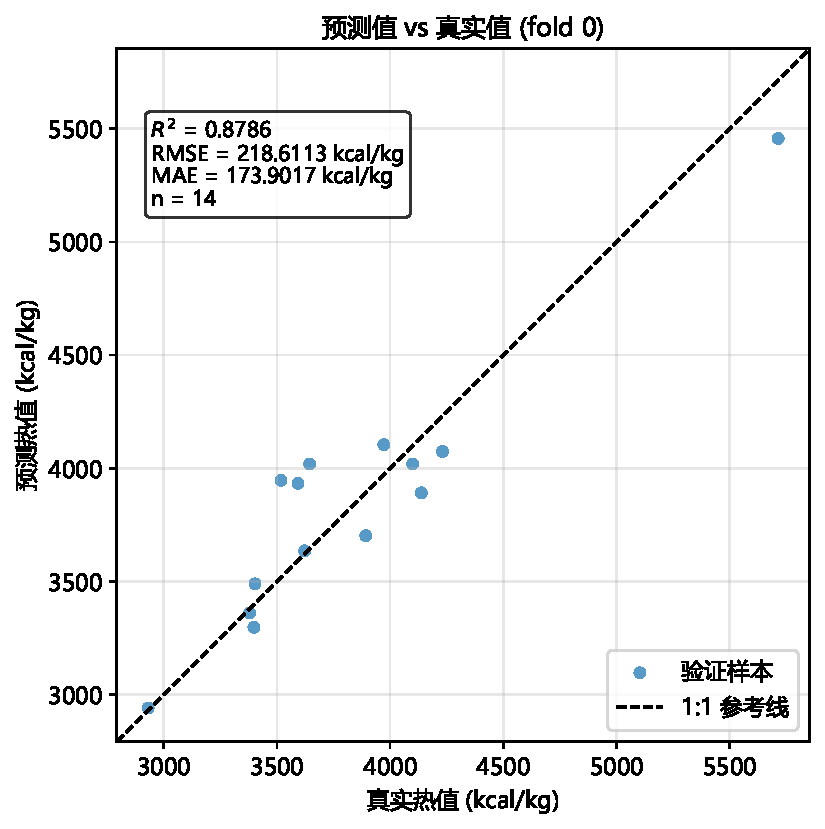
\includegraphics[width=0.65\textwidth]{fig_pred_true_fold0.pdf}
\caption{fold 0 验证集 hybrid 预测值 vs 真实值（1:1 参考线；$R^2=0.8786$，RMSE $= 218.6108$ kcal/kg，MAE $= 173.9012$ kcal/kg，$n=14$）。\label{fig:predtrue}}
\end{figure}

\begin{figure}[htbp]
\centering
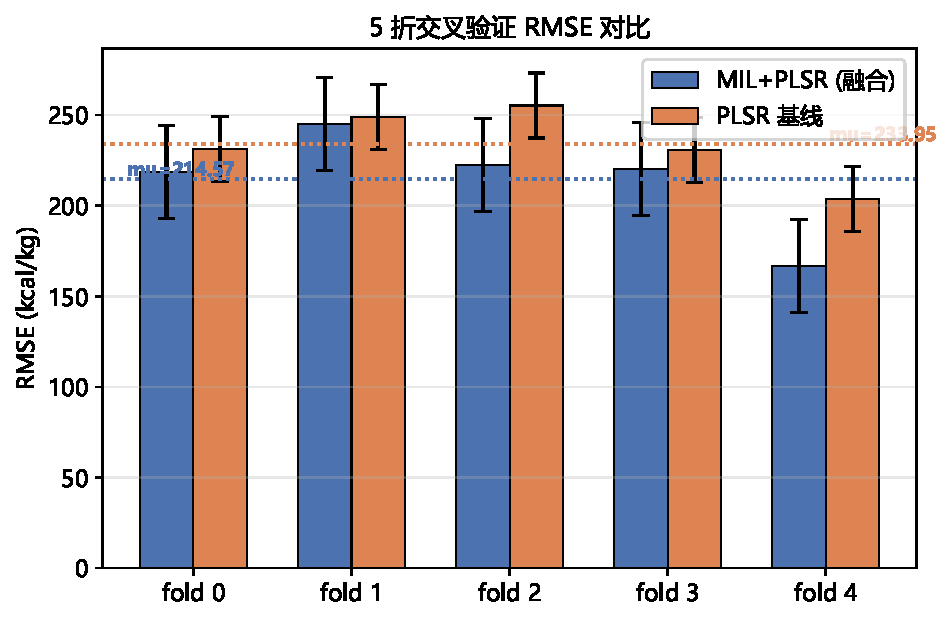
\includegraphics[width=0.78\textwidth]{fig_cv_rmse_bars.pdf}
\caption{5 折交叉验证 RMSE 对比：hybrid（MIL+PLSR，$214.57 \pm 25.71$ kcal/kg）vs PLSR 基线（$234.03 \pm 20.52$ kcal/kg）。\label{fig:cvrmse}}
\end{figure}

\section{结论}
\subsection{性能结论}
hybrid 融合预测在 5 折 bag 级交叉验证上全面优于 PLSR 基线：5 折 RMSE 均值 $214.57 \pm 25.71$ kcal/kg（$0.8978 \pm 0.1076$ MJ/kg），优于 PLSR 的 $234.03 \pm 20.52$ kcal/kg；fold 0 单折 $R^2 = 0.8786$，RMSE $= 218.6108$ kcal/kg，MAE $= 173.9012$ kcal/kg。最小残差 bag（bag 4）仅 $+12.86$ kcal/kg，最大正/负偏差分别来自 bag 6（$+427.98$ kcal/kg）与 bag 2（$-246.77$ kcal/kg），提示大颗粒原煤的单谱异质性仍是主要误差来源。

\subsection{可复现性与交叉校验}
将 5 折 RMSE 与项目官方 \texttt{summary.json} 交叉校验：
\begin{itemize}
  \item 官方记录均值（\texttt{official\_mean}）$= 214.5699$ kcal/kg；
  \item 本地从 5 折逐折重算均值（\texttt{recomputed}）$= 214.5699$ kcal/kg；
  \item 绝对差（\texttt{abs\_diff}）$= 1.1 \times 10^{-5}$ kcal/kg，落在数值舍入容差内，判定一致。
\end{itemize}
官方 \texttt{summary} 记录的模型标签 \texttt{method=pretrain+TransMIL\_attn}、\texttt{encoder=ResNet1D(base=16)+SupCon}、\texttt{fusion=FiLM(plsr\_dim=7)}、\texttt{n\_total\_params=924895} 与本报告第 2.2 节一致。综上，本报告的 5 折 RMSE 与均值指标可复现，未发生数值漂移。

\section*{数据与工具来源}
\begin{itemize}
  \item 推理与交叉验证：\texttt{mil-model} MCP 服务器（\texttt{cv\_summary}、\texttt{reproduce\_fold}、\texttt{predict\_calorific\_value}）；
  \item 绘图：\texttt{make\_figures.py}（matplotlib，保存 PDF 与 PNG 双格式）；
  \item 报告：\texttt{report} MCP 的本地 LaTeX 工具族（\texttt{write\_latex\_project}、\texttt{copy\_local\_file}）。
\end{itemize}

\end{document}